% !TeX spellcheck = en_US
\chapter{Error Functions}
As mention in \secref{sec:model-param-loss}, the loss function is the metric to assess the performance of the \ac{ML} model with a certain task. Different loss functions fit with different tasks. In many cases, the design of the loss function is what makes the differences.

\todo{Add graph and explanation}

\begin{figure}[!h]
	\centering
	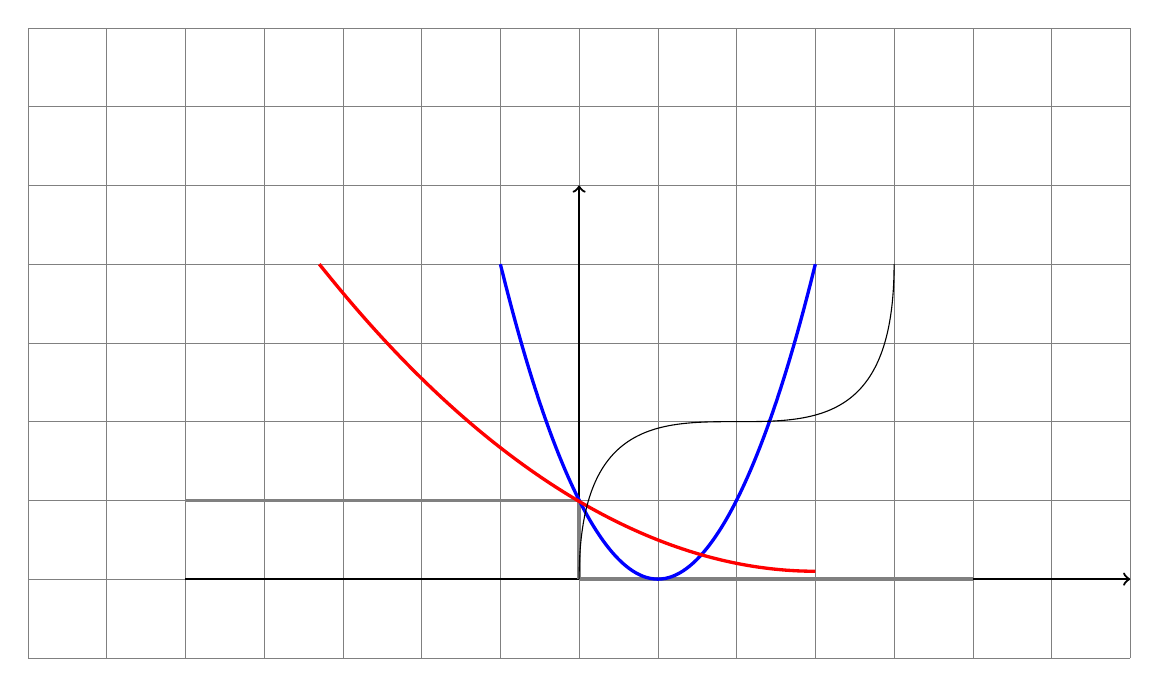
\begin{tikzpicture}		
		\draw[step=1cm,gray,very thin] (-7,-1) grid (7,7);
		\draw[thick, black, ->] (-5,0) -- (7,0);
		\draw[thick, black, ->] (0,0) -- (0,5);
		% Ideal miss-classification error		
		\draw[very thick, gray] (-5,1) -- (0,1);
		\draw[very thick, gray] (0,1) -- (0,0);
		\draw[very thick, gray] (0,0) -- (5,0);
		
		\draw[very thick, blue] (-1,4) parabola bend (1,0) (3,4);
		
		\draw[very thick, red] (3,0.1) parabola (-3.3,4);
		
		\draw (0,0) .. controls (0,4) and (4,0) .. (4,4);
		
	\end{tikzpicture}
	\caption{Different error functions: Ideal Miss-classification Error (gray line)}
\end{figure}

\section{Ideal Miss-classification Error}
Gradient = 0 $\Rightarrow$ can't use gradient descent.\\
It simply counts incorrectly classified points.

\section{Squared Error - $L_2$ Loss}
\begin{itemize}
	\item Leads to closed form solutions
	\item Sensitive to outliers
	\item Penalize "too correct" data points
\end{itemize}

\section{Cross Entropy Error}
\begin{itemize}
	\item Concave function $\Rightarrow$ unique minimum exists
	\item Robust to outliers, error increases only roughly linear
	\item No closed-form solution, requires iterative method
\end{itemize}

\section{Squared Error on Sigmoid / Tanh}
\begin{itemize}
	\item No penalty for "too correct" points
	\item Zero gradient for confidently incorrect classifications
\end{itemize}
$\Rightarrow$ \hlr{Do NOT} use $L_2$ loss with sigmoid outputs, instead, use cross-entropy.

\section{Hinge Error}
\begin{itemize}
	\item Robust to outliers
	\item Zero error for points outside margin $\Rightarrow$ sparsity
	\item Not differentiable around $z_n = 1$
\end{itemize}
\note Want the correct class to have a score that is higher than incorrect class by a fixed margin $\Delta$.
\begin{equation}
	L_i = \sum_{j \neq y_i} \text{max}(0, s_j - s_{y_i} + \Delta)
\end{equation}
in which, $s_j$ is other classes score, $s_{y_i}$ is real class score.

\section{$L_1, L_0$ Loss}
Median, no wrong points

\begin{align}
	&L_1 = \sum |t-y| \\
	&L_2 = \sum (t-y)^2
\end{align}

\section{Average Loss}
Mathematically, dividing the loss by the amount of data $N$ (in each batch or epoch) doesn't have any effect on the result. However, it's usually advisable to take the average to have more meaningful judgment and avoiding overflow when there are numerous data points.